% (C) 2020 Diogo Rodrigues
% Licensed under Creative Commons Attribution-NonCommercial-NoDerivatives 4.0 International (CC-BY-NC-ND 4.0)

\documentclass{sope}
\title{SOPE -- Exam 2017/18}
\author{Diogo Miguel Ferreira Rodrigues \\ \href{mailto:dmfrodrigues2000@gmail.com}{dmfrodrigues2000@gmail.com}}
\begin{document}

\setcounter{chapter}{17}
\exam{Exam 2017/18}
{
\renewcommand{\thesubsection}{\thesection\alph{subsection}}
\question{Question 1}
\begin{itemize}
    \item \textbf{Multiprogramming} is an operating system property which means it supports having several programs' code and data loaded in memory simultaneously.
    \item \textbf{Direct memory access} is an input/output technique where certain hardware subsystems (typically peripherals) can directly read from or write to main memory without CPU intervention. This means the CPU only needs to act in certain instants (to start and finish transactions), since the rest of the hard work (reads and writes to main memory) is done by the hardware subsystems, which have special access to particular parts of the main memory.
\end{itemize}
Multiprogramming and DMA are related since DMA is a very good way to free CPU time that can be used for improved multiprocessing. Also, multiprogramming and DMA allow the computer to simultaneously communicate with several hardware subsystems, since:
\begin{enumerate}
    \item DMA guarantees there can be several hardware subsystems directly writting to main memory at the same time;
    \item multiprogramming guarantees each hardware subsystem has direct memory access to a certain region, and all of them have simultaneous access so even if the system is single-process perypherals can fill in their dedicated memory regions anytime, and the CPU can fetch it from those special regions when it is ready to process it.
\end{enumerate}

\question{Question 2}
\questionitem{Item a}
The shared variable \texttt{pdata} should be declared as global, since \texttt{put} and \texttt{get} have no arguments referring to \texttt{pdata}, so they must access it via a global variable. \texttt{pdata} may be a pointer, which requires allocating heap memory with \texttt{malloc} in the main thread, before creating T1 and T2; it can otherwise be a global variable, in which case it has the advantages that it will be stored in the stack and will be in scope as long as the process is running, and it will also automatically fall out of scope (it will be deallocated) as the process ends. \par
\begin{lstlisting}[language=C]
semaphore items, slots, mutex;
PData pdata;

void* t1_thread_func(void *arg){
    while(should_produce()){
        PData *item = malloc(sizeof(PData)); produce(item);
        wait(slots);
        wait(mutex);
        put(item);
        signal(mutex);
        signal(items);
    }
    return NULL;
}

void* t2_thread_func(void *arg){
    while(should_consume()){
        wait(items);
        wait(mutex);
        PData item = get();
        signal(mutex);
        signal(slots);
        consume(item);
    }
    return NULL;
}

int main(){
    init(items, 0);
    init(slots, 1);
    init(mutex, 1);
    thread_t t1, t2;
    thread_create(&t1, t1_thread_func, NULL);
    thread_create(&t2, t2_thread_func, NULL);
    pthread_join(t1);
    pthread_join(t2);
    return 0;
}
\end{lstlisting}

\questionitem{Item b}
\textbf{(1)} False. A critical section is a piece of code that can only be executed by a single thread at all times. A piece of code that must be executed ininterrupted better corresponds to an atomic operation, which usually means it must be executed without context switch.\\
\textbf{(2)} In practice, a piece of code is made into a critical section by creating a mutex associated to that particular critical section, and have the mutex locked immediately before entering the critical section, and unlock the mutex immediately after exiting the critical section. This will guarantee only the thread that owns the mutex lock will be able to execute that section.

\questionitem{Item c}
Deadlocks may happen when all four of these conditions are met:
\begin{itemize}
    \item Mutual exclusion: only one process can use a resource at each instant.
    \item Hold and wait: a process can lock (hold) resources and then wait for more resources.
    \item No-preemption: a resource locked by a process can only be released by that process.
    \item Circular wait: the graph of resources and processes waiting for them has a cycle.
\end{itemize}
To stop deadlocks from happening, a programmer can either prevent or avoid them.
\begin{itemize}
    \item To prevent deadlocks, a programmer must make sure at least one of the abovementioned conditions does not hold.
    \item To avoid deadlocks, a programmer must implement the program so it doesn't provide resources to a process if that action at that specific time is considered a likely cause for a deadlock.
\end{itemize}
Usually the easiest way is to prevent deadlocks by carefully implementing the program so as to make one of the conditions false. One way to do this is to, for example, make sure the 2nd condition does not hold, by locking all resources before executing and releasing all resources if one of the demanded resources is already locked.

\question{Question 3}
\begin{center}
\begin{tabular}{p{25mm} | p{60mm} | p{60mm}}
    \textbf{Algorithm} & \textbf{Advantages} & \textbf{Disadvantages} \\ \hline
    First-Come First-Served & Simple, easy to implement, no starvation & Penalizes short and I/O-bound processes \\ \hline
    Shortest Job First / Shortest Remaining Time First & Optimal & Hard to implement, hard to estimate duration of the next CPU-burst, penalizes long processes \\ \hline
    Priority schedulling & & How to estimate priority? \\ \hline
    Round-Robin & No starvation, favours CPU-bound processes & Penalizes I/O-bound processes
\end{tabular}
\end{center}
There are two main axes for classifying processes, which amount to four groups:
\begin{itemize}
    \item Long vs short processes (in terms of total run time).
    \item CPU or I/O bound:
    \begin{itemize}
        \item CPU-bound: CPU-intensive, may have some very long CPU-bursts.
        \item I/O-bound: most time waiting for, or performing, IO. Typically has lots of short CPU-bursts.
    \end{itemize}
\end{itemize}
For instance, the FCFS algorithm tends to penalize short processes because they could be executed first in a very short time interval, but are instead put to the end of the queue, where they must wait for longer processes that arrived first. It also penalizes I/O-bound processes, because I/O devices end up having a very low usage (I/O-bound processes should be executed first to guarantee a decent I/O devices usage).

The SJB algorithm penalizes longer processes, typically by an excessive amount, since they end up at the end of the queue and may even be starved if several short processes arrive to the queue.

The RR algorithm penalizes I/O-bound processes in favour of CPU-bound processes, since they often block while waiting for I/O so they end up not using their quantum, being sent to the end of the queue they are forced to wait for quite a long time although they only used a small fraction of the quantum they were assigned.

\question{Question 4}
\questionitem{Item a}
Overlaying can be used for cases where program code is larger than available physical memory, but since it is not generic enough to apply for data as well I will be mentioning another technique.

Virtual memory is a generic method to execute processes that globally use more memory than available principal storage. Virtual memory is an abstraction of available memory, including primary storage and a part of secondary storage. At each instant, all process memory is mapped to virtual memory, but it can either physically be in primary or secondary storage, where blocks being currently used are in main storage and other blocks are in secondary storage, and blocks are swapped in and out of principal storage if other blocks are requested.

To make virtual memory possible, it is necessary to:
\begin{itemize}
    \item Divide process data and code into pages/segments.
    \item Have a real-time translator that converts virtual addresses into physical addresses.
    \item Have a swapping mechanism that allows moving pages between principal and secondary storage.
\end{itemize}

\questionitem{Item b}
It is important to know how certain programming structures are kept in memory to decrease access time, since memory management and page replacement algorithms can have a large impact in access time. This concept is better explained by examples.

A linked list is a linear sequential-access structure where an element points to the next element (it can additionally point to the previous element). This allows a relatively fast element insertion/removal anywhere in the structure, but it breaks the principle of locality of reference since a new element might be assigned to any one of the pages allocated to that process, so iterating over it can ultimately require swapping in and out pages just to access a single element, causing trashing.

An array has better locality of reference because elements are assigned to contiguous memory addresses, so iterating over an array is faster because a new page has to be loaded only when the array is too large to fit in a single page, and even so the number of swaps is generally very low.

However, if one has a matrix as an array of arrays, one has to take care that the elements that are contiguous in memory are those in the second dimension, so option 1 is faster than option 2 because in option 1, for each \texttt{i} we access the contiguous elements \texttt{M[i][:]} which are in the same array, but option 2 consecutively accesses elements in different arrays (\texttt{M[i][j]} and \texttt{M[i+1][j]} are in different arrays, \texttt{M[i][:]} and \texttt{M[i+1][:]} respectively) which might be allocated in different pages, which can lead to the worst case where elements being consecutively accessed are in different pages, causing trashing.

\begin{lstlisting}[language=C]
// Option 1
for(int i = 0; i < M; ++i)
    for(int j = 0; j < N; ++j)
        doMath(M[i][j]);
// Option 2
for(int j = 0; j < N; ++j)
    for(int i = 0; i < M; ++i)
        doMath(M[i][j]);
\end{lstlisting}

In sum, the principle of locality of reference (on which paging algorithms depend to have the best possible performance) is best kept if elements are consecutively stored in memory in an order that most resembles the order by which they will be accessed; an array has consecutive elements in memory and a list does not, and a matrix being accessed through option 2 does not follow the same order elements are stored in memory (which are contiguous with other elements by just varying the second dimension).

\question{Question 5}
Files can be stored in non-contiguous memory blocks, so to make sense of them Linux uses \emph{inodes}, which are entries in the special table called \emph{active inodes table}, where each inode registers some file metadata along with the memory blocks the file was saved to (and their order), so an inode has the job of being the \emph{actual file} and making sense of the blocks in memory.

Directories are special files that map names of files to inodes, so several file names can be mapped to the same \emph{actual file}/inode (thus making them all hard links).

\newpage
\question{Question 6}
\questionitem{Item a}
\lstinputlisting[language=C,firstline=59,lastline=71]{2018N_06.c}

\questionitem{Item b}
\lstinputlisting[language=C,firstline=20,lastline=40]{2018N_06.c}

\newpage
\questionitem{Item c}
\lstinputlisting[language=C,firstline=41,lastline=53]{2018N_06.c}

\textbf{File:} \texttt{2018N\_06.c}
\lstinputlisting[language=C]{2018N_06.c}
\textbf{File:} \texttt{2018N\_06.sh}
\lstinputlisting[language=bash]{2018N_06.sh}
\textbf{Directory tree:}

\dirtree{%
.1 2018\_06\_testdir.
    .2 src.
        .3 hello.
            .4 imonefile.txt.
        .3 hey.
            .4 another.
                .5 anotherfile.txt.
                .5 notafil.txt.
            .4 afile.txt.
    .2 dst.
        .3 afile.txt.
        .3 anotherfile.txt.
        .3 imonefile.txt.
}

\question{Question 7}
\questionitem{Item a}
\begin{center}
    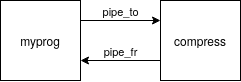
\includegraphics[scale=0.5]{2018N_07_a}
\end{center}
\lstinputlisting[language=C,firstline=10,lastline=30]{2018N_07_a.c}

\questionitem{Item b}
\begin{center}
    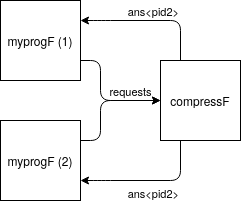
\includegraphics[scale=0.5]{2018N_07_b}
\end{center}
\lstinputlisting[language=C,firstline=23,lastline=59]{2018N_07_b.c}

\questionitem{Item c}
POSIX requires writes of size less than \texttt{PIPE\_BUF} must be atomic, where \texttt{PIPE\_BUF} must be at least $\SI{512}{\byte}$, but in Linux \texttt{PIPE\_BUF} is $\SI{4096}{\byte}$. If the \texttt{data} field had a size of $\SI{100000}{\byte}$, then the struct write will require the writting of more than \texttt{PIPE\_BUF} bytes, meaning the operation is not guaranteed to be atomic. Atomicity guarantees there will not be interleaved data (data from different write instructions ending up mixed together because there is a chance one of the writes was blocked to change context). The fact there is no atomicity guarantee for this case means there can be an interleaving problem, which breaks message integrity as read operations need to make assumptions (first the number of bytes is read, and then that number of bytes is expected to be an incorrupted message).

\question{Question 8}
\questionitem{Item a}
\lstinputlisting[language=C,firstline=38,lastline=47]{2018N_08_a.c}

\questionitem{Item b}
\lstinputlisting[language=C,firstline=24,lastline=38]{2018N_08_a.c}

\questionitem{Item c}
\lstinputlisting[language=C,firstline=13,lastline=27]{2018N_08_c.c}
For \texttt{bird} to work correctly, \texttt{baby} will have to use the mutex and the conditional variable that \texttt{bird} uses, otherwise there is not synchronization. Namely, \texttt{baby} will have to lock \texttt{food\_bits\_mutex} to write to it, and will have to signal \texttt{cond} when it eats a bit (thus decrementing \texttt{food\_bits}). It can also use the conditional variable \texttt{cond} to avoid a busy-wait when waiting for \texttt{bird} to get more food.

\newpage
Although the problem statement requires to explain only by words, we also present a sample solution for \texttt{baby}:
\lstinputlisting[language=C,firstline=29,lastline=46]{2018N_08_c.c}

\questionitem{Item d}
\lstinputlisting[language=C,firstline=45,lastline=47]{2018N_08_d.c}
\lstinputlisting[language=C,firstline=58,lastline=64]{2018N_08_d.c}

}

\end{document}